\section{Introduction}\label{sec:1}

Online hiring platforms process millions of resume--job pairs annually, and the systems that rank them are increasingly load-bearing for both the candidate and the recruiter \citep{tang2025explainable}.
A typical applicant tracking system (ATS) receives a resume, parses it into a structured representation, scores the resume against an open job requisition, and returns a ranked shortlist.
The scoring function is, in the dominant production paradigm, a single number with no breakdown of which resume fields or job requirements drove the rank \citep{koren2009matrix,he2017neural}.
This opacity is not an oversight; it is the cost of optimizing for offline ranking metrics at scale, and the cost is paid by the people whose careers depend on the output.

\subsection{The engineering problem}\label{sec:1.1}
The recruitment domain has a documented accountability gap that follows directly from opaque ranking.
A recruiter who has shortlisted 20 candidates from a pool of 200 cannot, with the current generation of ATS tools, point to the specific job requirements that moved a candidate into or out of the shortlist.
A candidate who has edited a resume to add a new skill has no way to see whether the new skill moved a posting up or down the list, or whether the change reached the system at all.
A compliance officer who needs to audit a hiring decision for disparate-impact liability under equal-employment law \citep{raub2018bots,ajunwa2021paradox} has no access to the per-decision factor decomposition that would make the audit tractable.
The accountability gap is an engineering problem with a known cost: time-to-hire rises when recruiters must verify shortlist decisions manually, candidate satisfaction drops when applicants cannot act on opaque rankings, and the regulatory exposure of the platform grows when the scoring function is not auditable.

\subsection{Regulatory and engineering context}\label{sec:1.2}
The accountability gap is not hypothetical.
Recent regulatory frameworks in the European Union, the United Kingdom, and several US jurisdictions have begun to require auditable explanations of algorithmic decisions that affect employment outcomes \citep{raub2018bots,ajunwa2021paradox}.
This growing scrutiny makes auditability and per-decision documentation increasingly important for algorithmic systems that affect employment decisions; and the cost of retrofitting an auditable explanation layer onto a deployed opaque system is typically higher than the cost of designing for auditability from the start. We do not claim compliance with any specific statutory provision --- establishing that is a legal question beyond this paper's scope --- only that decomposable, documented decisions are the engineering prerequisite for such audits.
The engineering cost of opaque ranking is also concrete: verifying shortlist decisions manually consumes a substantial share of recruiter time, and candidates on platforms that expose no per-decision feedback have no actionable signal for how to improve their standing (we state these as qualitative motivations, not measured effects).
These costs are the motivation for the present work: an applied AI system that integrates the per-decision factor decomposition, the calibrated confidence, and the explanation generation into a single inference, so that the auditability and the user-facing transparency are properties of the inference itself rather than properties of a post-hoc attribution step.

\subsection{Limitations of existing AI approaches}\label{sec:1.3}
Existing AI approaches to the recruitment ranking problem fall into three families, each with a known limitation.
\emph{Learned-to-rank systems} \citep{he2017neural,covington2016deep,koren2009matrix} optimize for offline metrics (nDCG, MAP, MRR) on historical interaction data and return a single score.
They are accurate on aggregate metrics but opaque on individual decisions, and they are not auditable without a separate attribution step.
\emph{Neural semantic matchers} \citep{reimers2019sentence} encode resumes and job descriptions into a shared embedding space and return a similarity score.
They are flexible and language-aware but treat the score as a black-box number and do not decompose the score into interpretable factors.
\emph{LLM-based systems} \citep{wei2022chain,yao2023react,sumers2024cognitive} are increasingly used for resume parsing, job description normalization, and explanation generation, but they are not yet used as the primary ranker in production systems; their latency, cost, and non-determinism are blocking issues for the hot path of a high-throughput ATS.

\subsection{Why current approaches are insufficient}\label{sec:1.4}
The three families share a common limitation: none of them returns, in a single inference, a ranked list with both per-decision factor decomposition and a calibrated confidence value.
The factor decomposition is what makes an explanation auditable; the calibrated confidence is what makes a confidence display trustworthy.
A ranking system that returns only a single number requires a separate attribution step (which is post-hoc, not part of the inference) and a separate calibration step (which is not part of the inference either), and the two steps may not be consistent.
A ranking system that integrates the factor decomposition and the calibrated confidence into the inference itself is a more reliable engineering artifact, and the engineering benefit compounds when the inference also includes an explanation that is anchored to the same factors.

\subsection{Research gap}\label{sec:1.5}
The research gap is a lack of applied AI systems for the recruitment domain that integrate three properties in a single inference: a multi-channel composite ranking with factor decomposition, a calibrated confidence value, and a component-level explanation that is bound to the channels that produced the score.
Existing systems address one or two of the properties but not all three.
A production-grade recruitment ranking system requires all three because the recruitment workflow is a multi-stakeholder decision process (candidate + recruiter + compliance) in which each stakeholder requires a different view of the same ranking.

\subsection{Our contribution}\label{sec:1.6}
We address this gap with \JobMatch, an auditable, calibrated, and explainable recommendation methodology for the recruitment domain, implemented as a modular multi-agent system (the agent decomposition is an engineering/failure-isolation choice, not the scientific contribution; see \secref{sec:5.7}).
The architecture decomposes the ranking workflow into a small set of role-separated components, each with a single user constituency and a clearly defined interface to the others.
The contribution is fourfold:
\emph{(i)} A composite ranking with six explicit channels (semantic similarity, skill overlap, title fit, experience tier, compensation fit, remote policy), each contributing a documented weight, enabling component-level explanations without post-hoc attribution; and, for the skill channel, a graded relation-aware matcher (exact/related/unrelated with partial, never full, credit for related skills) defined in \secref{sec:3} and evaluated in \secref{sec:5.7} on a de-circularized benchmark.
\emph{(ii)} A calibrated confidence display that applies Platt scaling \citep{platt1999probabilistic,guo2017calibration} to the composite ranking output and reports a confidence value alongside the ranked list, reducing the held-out 5-fold expected calibration error to 0.019, while we report that the calibrated confidence has limited discrimination (a stated limitation).
\emph{(iii)} An automated, component-level faithfulness evaluation suite (structural checks plus a mechanistic ranking-level probe, not a human faithfulness study) that quantifies whether explanation bullets correspond to the channels that produced the score, and a counterfactual probe that tests whether single-field edits predicted by the explanation move the rank.
\emph{(iv)} A reproducible engineering surface: the prototype, the frozen demo corpus (30 resumes, 15 jobs, 47 labeled pairs), the explanation generator, the calibration layer, and a 341-test regression-gated benchmark are released as an open-source artifact.

\begin{table*}[t]
\centering
\small
\caption{The contribution at a glance: each claimed contribution, the mechanism that realises it, and how it is evaluated in this paper. The novelty is the auditable \emph{integration} and its property-by-property evaluation, not a new ranking algorithm.}
\label{tab:contrib}
\begin{tabular}{@{}lll@{}}
\toprule
Contribution & Mechanism & Evaluation \\
\midrule
Decomposable ranking     & six explicit weighted channels (fixed priors)      & nDCG@5 + leave-one-channel ablation (\secref{sec:5.1}) \\
Relation-aware skills     & exact / related / unrelated graded credit          & de-circularized skill benchmark + decomposition (\secref{sec:5.7}) \\
Calibrated confidence     & Platt / beta / isotonic on the composite score     & ECE + adaptive ECE + Brier skill + AUC (\secref{sec:5.3}) \\
Explanation faithfulness  & score-bound templates + mechanistic probe          & structural checks + rank-displacement probe (\secref{sec:5.2}) \\
Counterfactual robustness & controlled single-field profile edits              & rank / score sensitivity (\secref{sec:5.4}) \\
Reproducibility           & frozen artifacts + one-command CI gate             & 341 regression tests, verifier-gated numbers (\secref{sec:5}) \\
\bottomrule
\end{tabular}
\end{table*}

\subsection{Application context}\label{sec:1.7}
\figref{fig:app} shows the prototype candidate-side portal in operation: the candidate has uploaded a resume, the system has parsed and normalized the profile, and the ranked list of jobs is returned with the per-decision factor decomposition (semantic fit, skills overlap, experience fit, compensation fit, remote fit), the calibrated confidence, and the matched and missing skill tokens visible inline.
\figref{fig:app2} shows the symmetric prototype employer-side portal: the recruiter has pasted a job description, the system has parsed the requirements, and the ranked list of candidates is returned with the same factor decomposition and a per-candidate explanation drawer.
\figref{fig:portal-survey} gives a comprehensive view of the same portal surface, covering all eight primary interaction states in the order a user encounters them: candidate-side (a) resume upload, (b) parsed-fields confirmation, (c) match list with explanation, and (d) counterfactual view; employer-side (e) job upload, (f) requirements confirmation, (g) reverse match list, and (h) shortlist panel.
A candidate or recruiter interacts with a transparent interface that surfaces the per-decision factor decomposition and the calibrated confidence alongside the ranked list.
The system is a research prototype rather than a production deployment; the application consequence is the engineering pattern, not a specific commercial product.
\figref{fig:hld} shows the high-level architecture; \figref{fig:candidate-pipeline} and \figref{fig:employer-pipeline} expand the candidate- and employer-side components; \figref{fig:capstone} adds the admin/evaluation console and the data plane.

\begin{figure*}[!t]
\centering
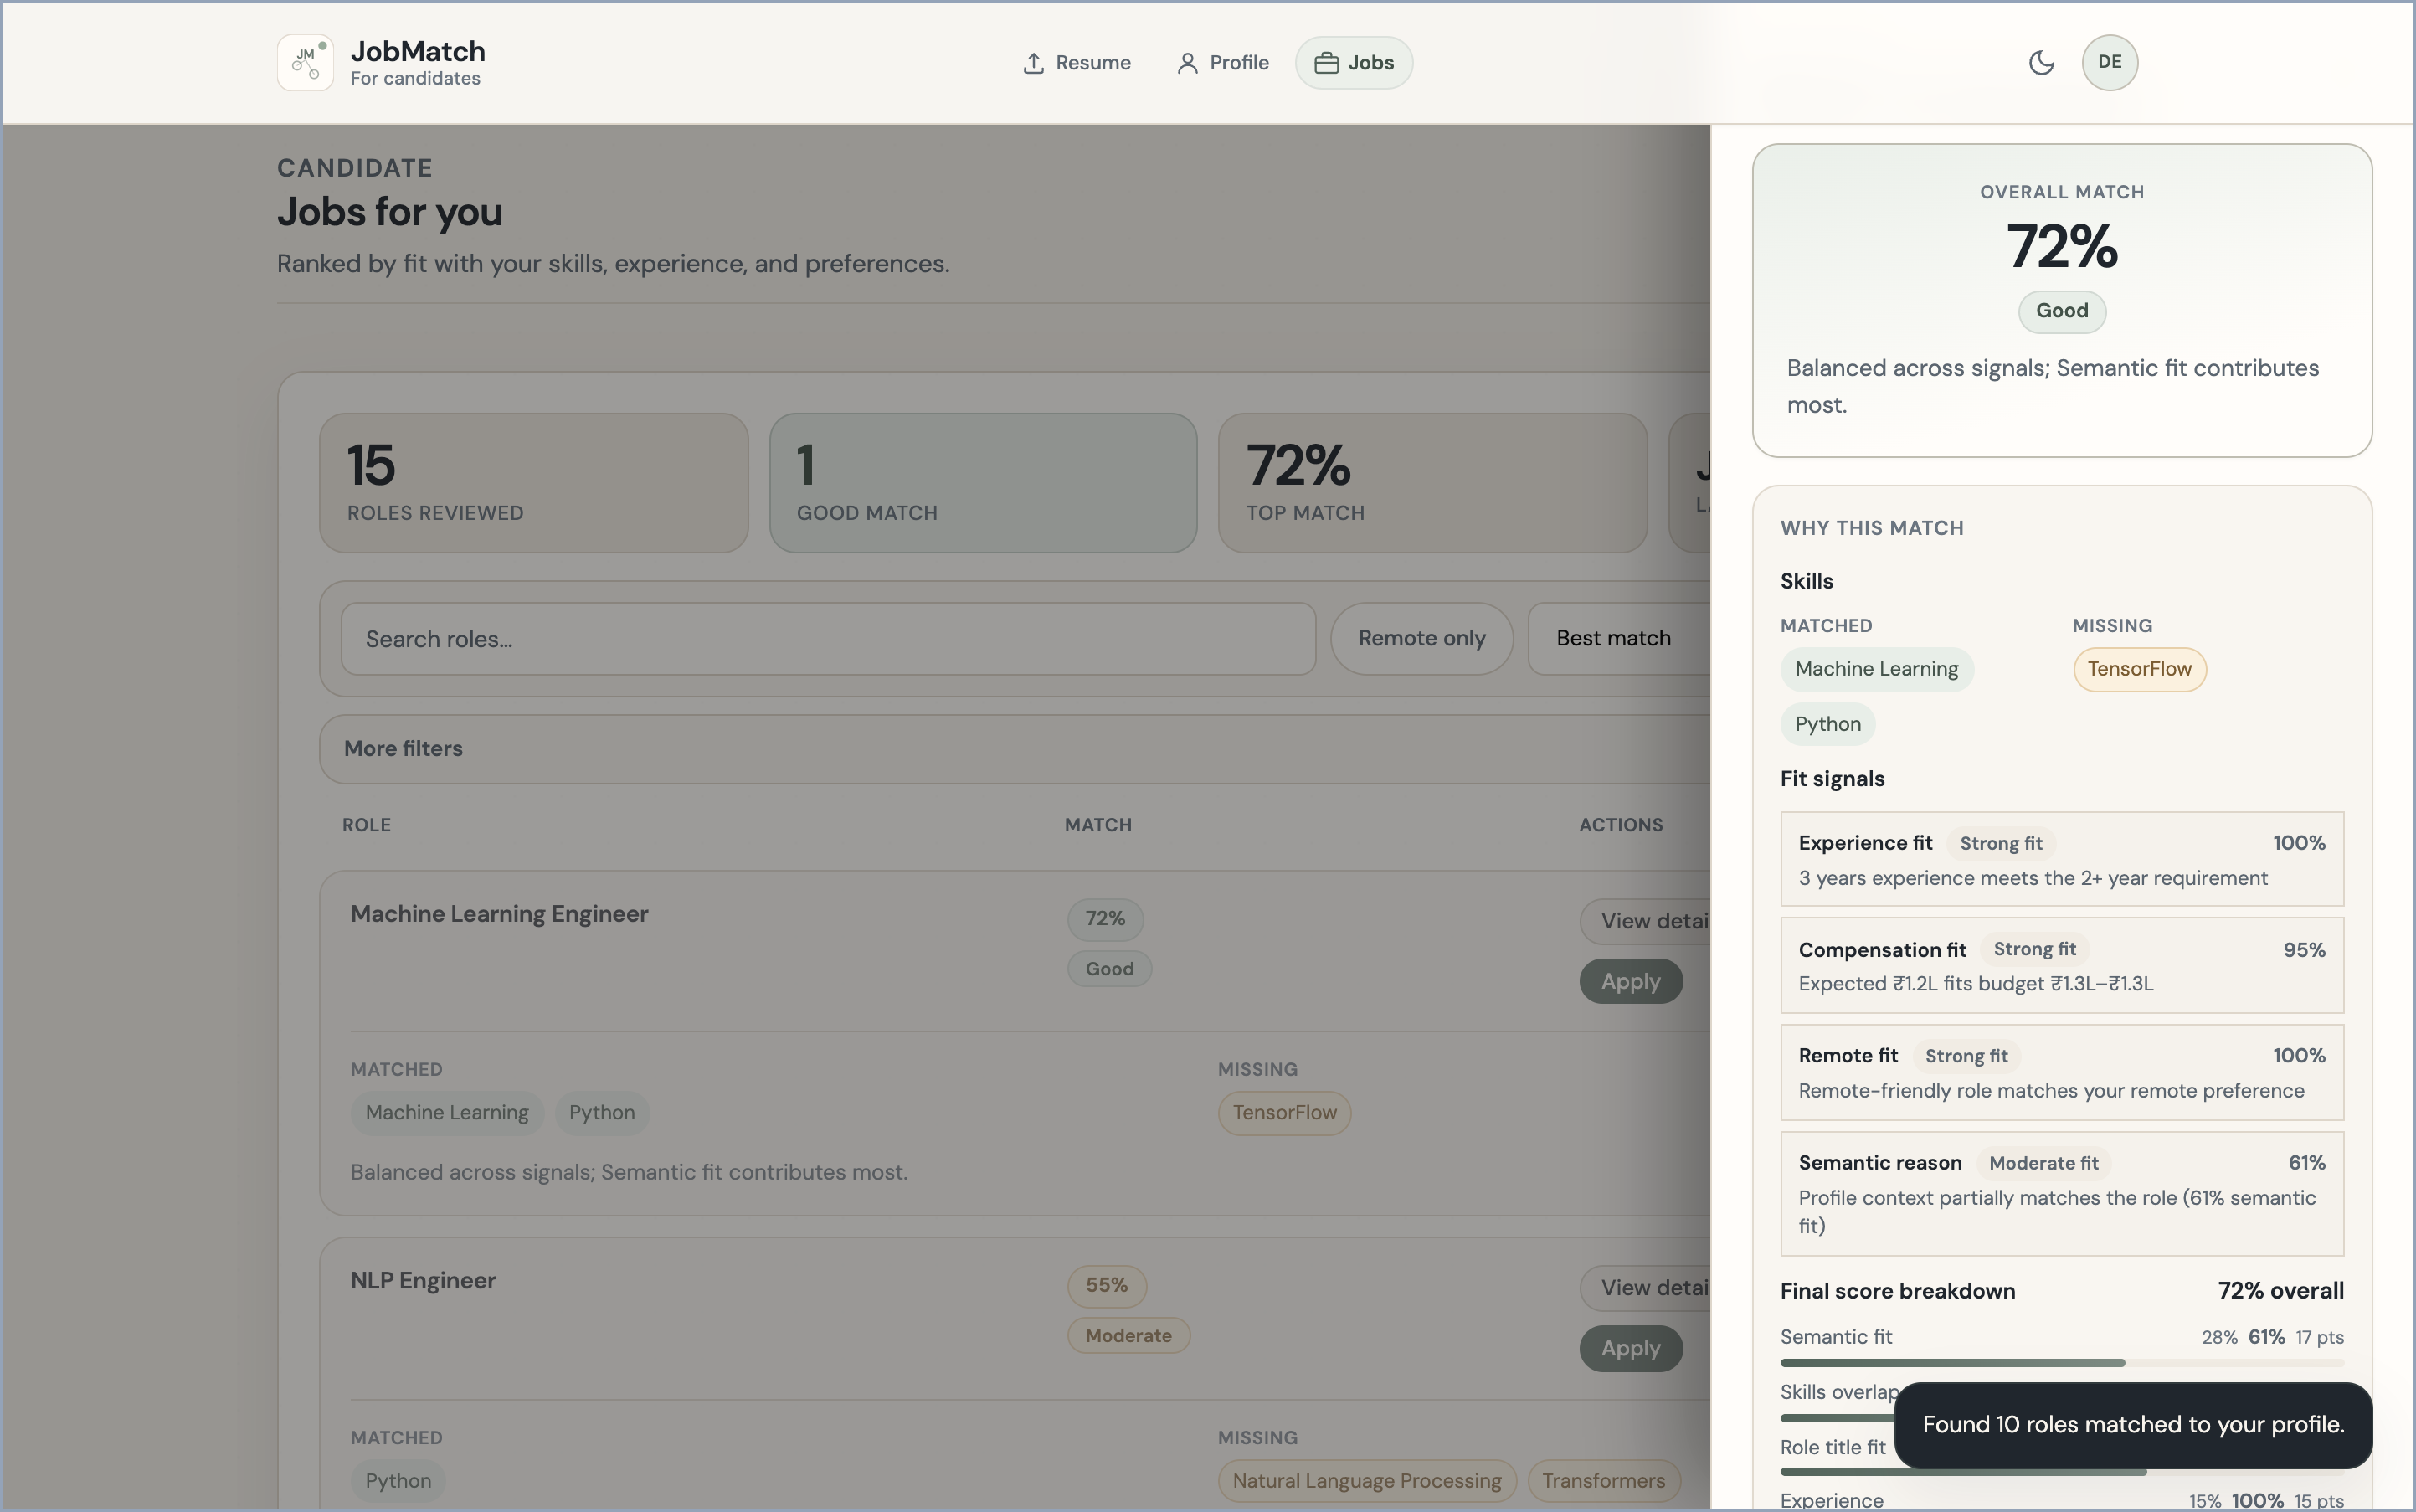
\includegraphics[width=0.95\linewidth]{figures/fig1_application.png}
\caption{Prototype candidate-side portal: ranked job list with the per-decision factor decomposition (skills overlap, experience, compensation, remote, semantic) and the calibrated confidence (72\%, "Good") shown both as a header and as an expandable drawer on the right of the selected job. Matched skill tokens (Machine Learning, Python) and missing tokens (TensorFlow) are surfaced inline so the candidate can act on the output without leaving the page.}
\label{fig:app}
\end{figure*}

\begin{figure*}[!t]
\centering
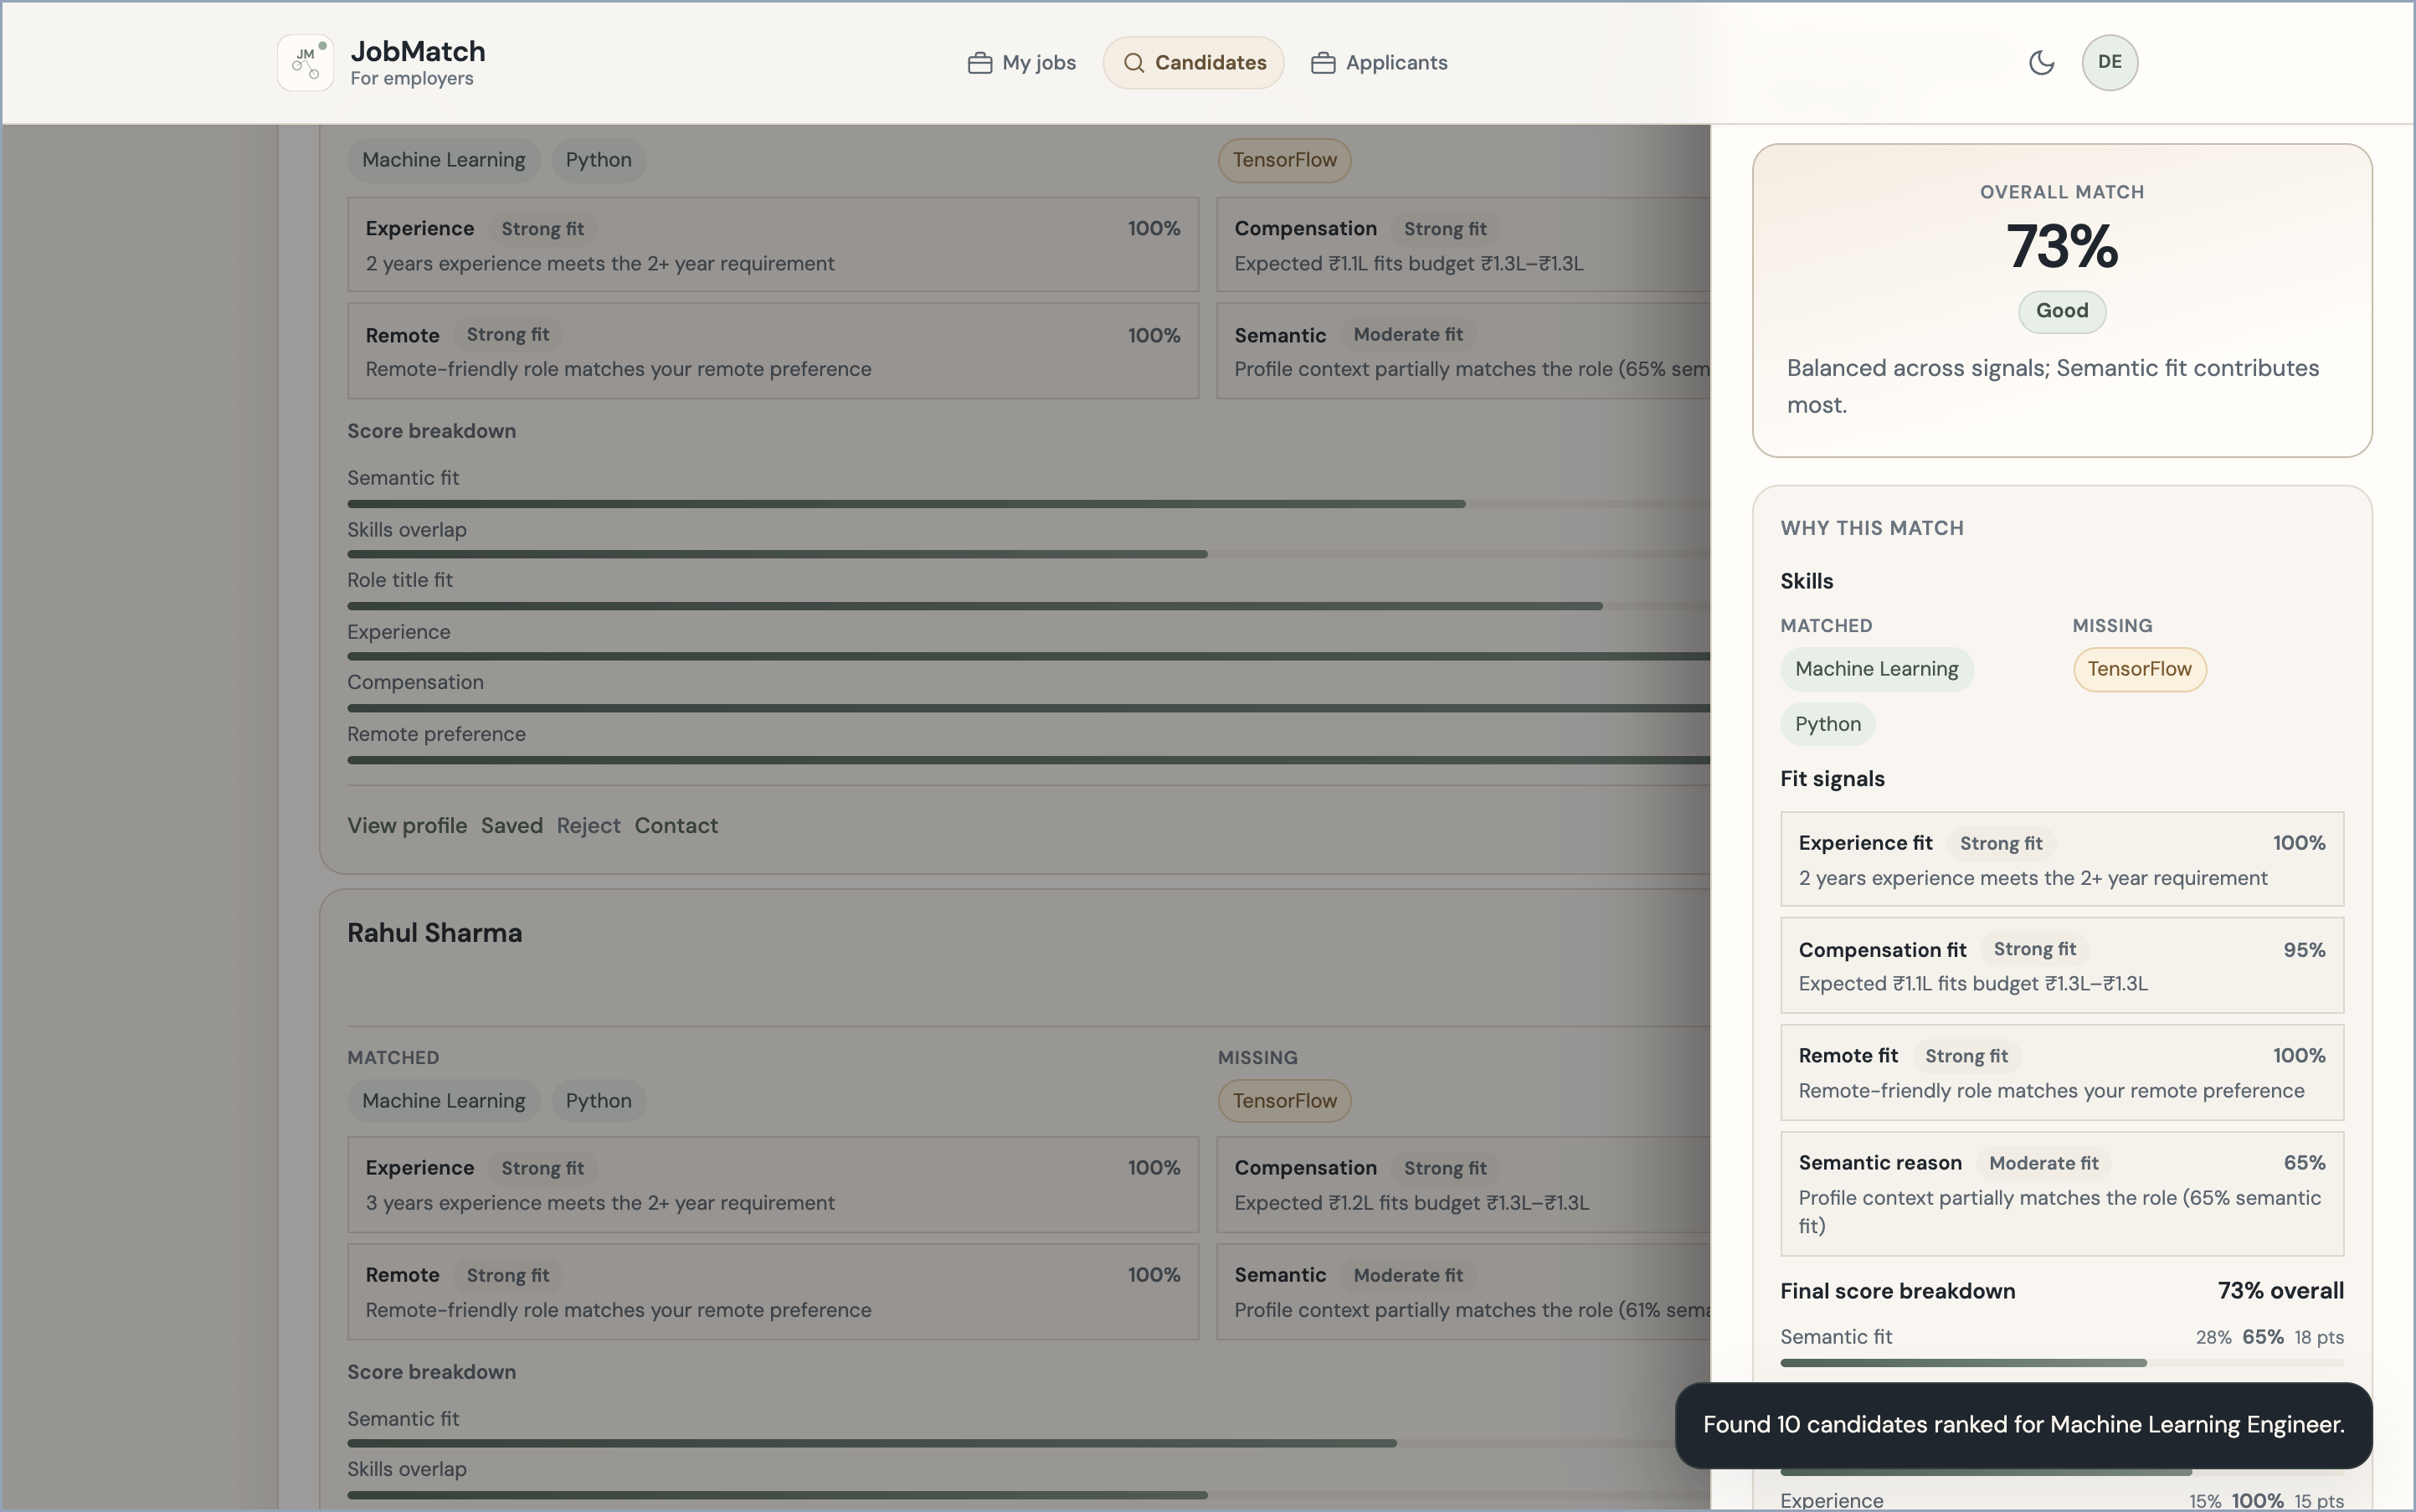
\includegraphics[width=0.95\linewidth]{figures/fig2_employer_view.png}
\caption{Prototype employer-side portal (reverse direction): ranked candidate list for a posted job, with the per-candidate factor decomposition (semantic, skills, experience, compensation, remote), the per-candidate calibrated confidence, and the inline action menu (view profile, saved, reject, contact). The recruiter sees the same explanation structure that the candidate sees; the scoring pipeline is symmetric and the only difference is the direction of the query.}
\label{fig:app2}
\end{figure*}

\begin{figure*}[!t]
\centering
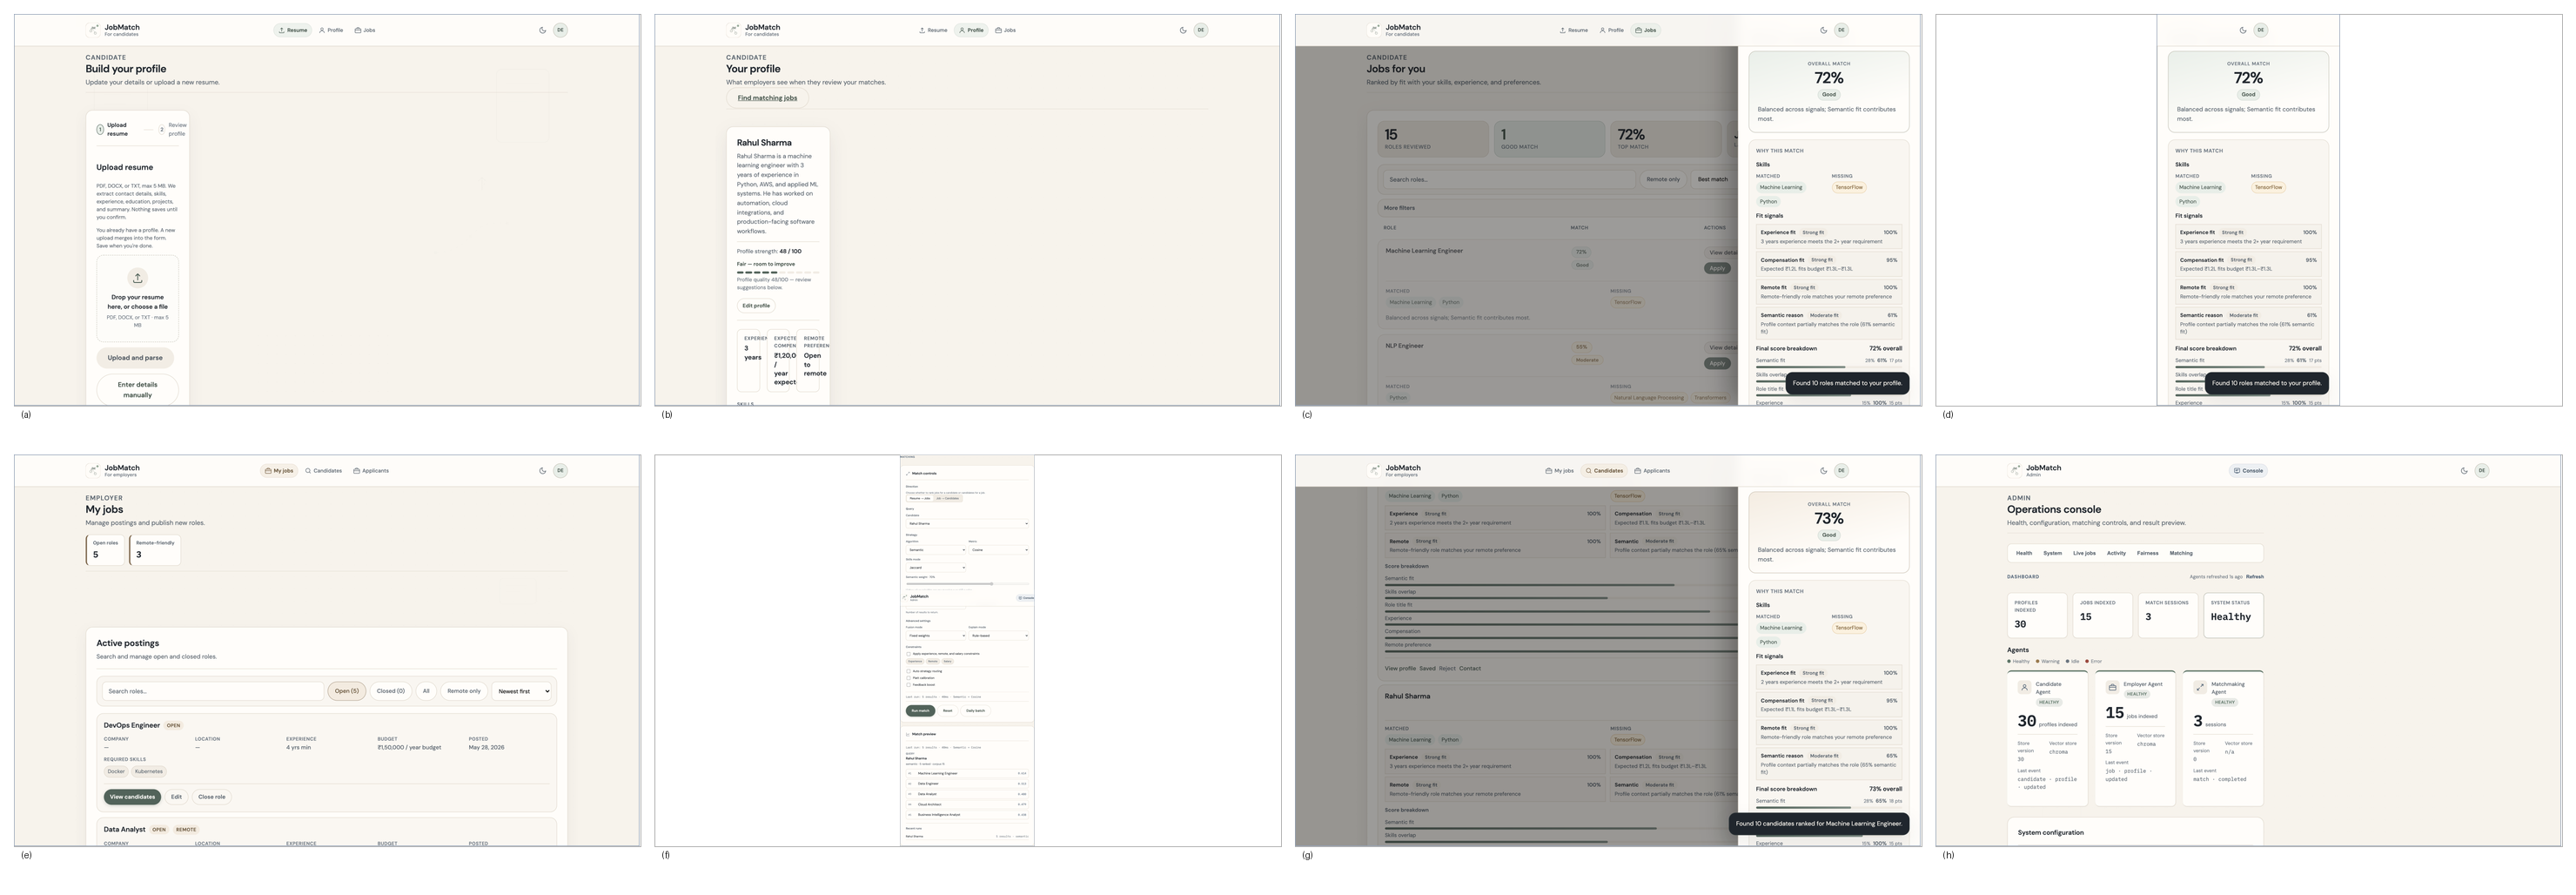
\includegraphics[width=0.92\linewidth]{figures/Fig10.png}
\caption{Comprehensive view of the prototype portal surface, showing all eight primary interaction states in the order a user encounters them. Top row (candidate side): (a) resume upload and review; (b) parsed-fields confirmation; (c) match list with component-level explanation drawer; (d) counterfactual view showing how a small edit to a snapshot field would move the rank. Bottom row (employer side): (e) job-description upload and review; (f) parsed-requirements confirmation; (g) reverse match list with component-level explanation; (h) shortlist panel. The admin/evaluation console (event strip, agent health, manual match, demo reset) is not shown here. The single-state views of Figs.~\ref{fig:app} and~\ref{fig:app2} correspond to panels (c) and (g) of this figure.}
\label{fig:portal-survey}
\end{figure*}

\begin{figure*}[!t]
\centering
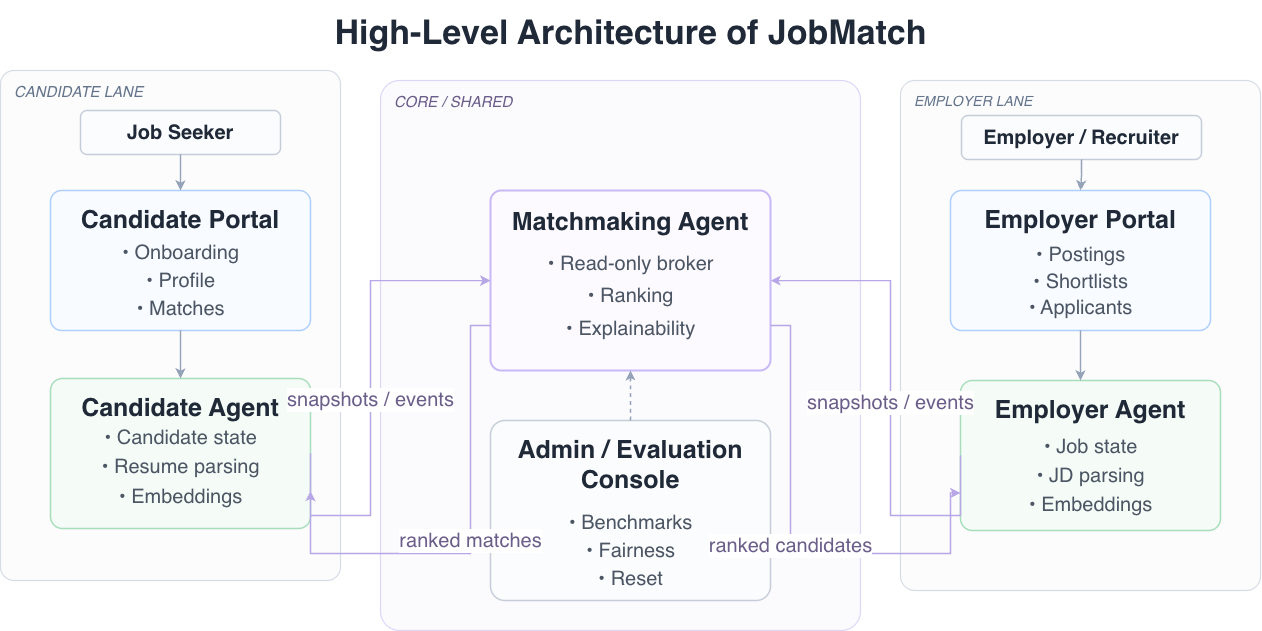
\includegraphics[width=0.95\linewidth]{figures/Fig1.png}
\caption{High-level layout of \JobMatch. The candidate-side component (C1) and the employer-side component (C2) own the user-editable state on each side of the market. The matchmaking component (C3) reads those snapshots, returns a ranked list with component-level reasons and a calibrated confidence, and never writes into either store. The dashed arrows represent snapshot and event flow; the solid arrows represent user-facing recommendations and feedback. The portals shown above (Figs.~\ref{fig:app} and~\ref{fig:app2}) are two of the three role-specific portals (candidate, employer, administrator) sharing the same scoring and explanation pipeline.}
\label{fig:hld}
\end{figure*}

\subsection{Paper organization}\label{sec:1.8}
The remainder of the paper is organized as follows.
\secref{sec:2} reviews the literature on AI-based recommendation, semantic matching, knowledge-driven AI, LLM agents, explainable AI, and trustworthy AI.
\secref{sec:3} describes the proposed methodology, including the multi-agent architecture, the knowledge representation, the composite ranking, the explanation generation, the confidence calibration, and the implementation details.
\secref{sec:4} describes the experimental setup, including the corpus, the baselines, the metrics, and the evaluation protocol.
\secref{sec:5} reports the results, including the main ranking comparison, the faithfulness evaluation, the calibration results, the counterfactual probe, and the ablation study.
\secref{sec:6} discusses the engineering implications and the limitations of the evaluation.
\secref{sec:7} outlines the future work.
\secref{sec:8} concludes.
